\section{Methods}
The following section will first give an explanation of what federated learning is and how it works, then detail how we used the \enquote{COVID-19 detection using federated machine learning} paper\cite{federated_machine_learning} to test and implement it in our research and lastly also give a short overview of the goals and methods of papers we tried to replicate and modify.

\subsection{Federated Learning}\label{subsec:methods_federated_learning}
Federated learning was first introduced by Google on their Google AI blog as a way to do \enquote{Collaborative Machine Learning without Centralized Training Data}\cite{google_ai_federated_learning}. The initial intention behind its development was to enable low power devices like mobile phones to collaboratively train a shared machine learning model without the need to keep all of the training data somewhere in the cloud and accessible to all devices. Another benefit of training models on client devices is that they can instantly be used for prediction as well, which lowers time overhead in comparison with models that are queried over the internet on a central server and even continues to work if there is no internet connection available.
Figure \ref{fig:google_ai_fl} shows the basic idea of federated learning. 

\begin{enumerate}
    \item First, a shared model is initialized and distributed to client devices (or directly initialized on device).
    \item The local model is trained with data on the device. [A]
    \item All local models are combined to update the shared model. [B] 
    \item The shared model is then redistributed to all clients, where it gets trained further with local data. [C]
\end{enumerate}

\begin{figure}
    \centering
    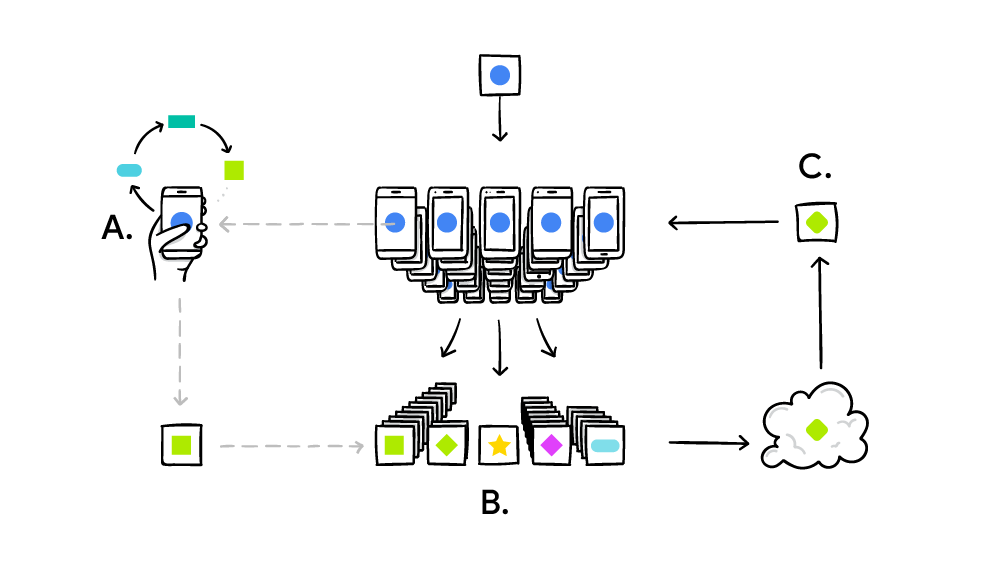
\includegraphics[width=1.0\linewidth]{imgs/FederatedLearning_googleai.png}
    \caption{Federated learning overview by Google AI.\cite{google_ai_federated_learning}}
    \label{fig:google_ai_fl}
\end{figure}

With this process it is not only possible to utilize low-power devices for training machine learning models but also to use and keep private data on the device, protecting privacy as the only data that is transmitted to the central server are the model updates in form of its weights. The local weight updates can then be deleted once incorporated into the shared model.

non-iid data

same drawbacks than any other communication based algorithm: small amount of clients, dropped connections, general variability of conditions 
-> quickly describe save methods of sharing data (differential privacy, encryption, etc)

Not only mobile devices, but: organizations, IoT, healthcare organizations / governments

\subsubsection{Federated Averaging}
communication overhead:
FedSGD vs FedAvg


\subsection{Implementing Federated Learning}\label{subsec:methods_original_paper}
To get started, we wanted to use the \enquote{COVID-19 detection using federated machine learning} paper\cite{federated_machine_learning}, also named the \textit{federation paper} from here on out, and (re)build the sequential and federated models described by the authors to learn how this collaborative process is implemented in real world scenarios. The main reason we decided to use this exact paper is, that it has the same goal of testing federated learning in Covid research and that at the time of searching for a project topic, it was one of the only ones available doing this and also having a public dataset available.
There is no public code of the original implementation available, but a step-by-step description of the authors process is included. The paper uses the Tensorflow Federated framework\cite{tensorflow_federated} and assumes that the reader has some knowledge of Tensorflow, Keras and Tensorflow Federated. Because of this assumption, the steps were not detailed enough for us to properly reproduce their solution, which is why we decided to build our own training environment in PyTorch and use its pre-build ResNet18 as the model of choice. Training and test data, a Kaggle dataset\cite{}, as well as data preprocessing was done the same way as described in the paper. The authors tested both SGD and Adam optimizers and found that SGD outperformed Adam very slightly. However, in our own initial tests Adam performed better and we consequently only used it as the optimizer in our implementation.

In real federated scenarios the clients are deployed on different hardware and have to communicate extensively with each other in order to update their respective models. While this is an important part of federated learning in real world scenarios, it is not directly a machine learning problem. Network communication is a complete research topic in itself and as described in section \ref{subsec:methods_federated_learning} there already exist algorithms and ideas specifically tailored to make the communication part in federated learning as efficient and secure as possible. For this reason and in correspondence with following the paper example, we decided that the learning and not the communication part is of more interest and relevance to the task at hand and therefore opted to not train our client models on separate machines. They are rather implemented as different and strictly isolated instances of the same model on the same computer, which makes copying and aggregating their model weights easier while still maintaining the core parts of federated learning (minus the network communication).

\subsection{Overview of Adapted Papers}\label{subsec:methods_adapted_papers}
After the first paper proved hard to replicate exactly, we chose to only adapt papers where code is publicly available. This also makes verifying and comparing our results with the authors results much easier.
To make the lessons learned from the \textit{federation paper} applicable, all models discussed and implemented also use some form of image data for Covid-19 identification.

\paragraph{COVIDNet}
\paragraph{DLH-Covid}
\paragraph{DarkCovidNet}
\paragraph{GraphCovidNet}